\documentclass{article}
\usepackage[utf8]{inputenc}
\usepackage[french]{babel}

\textwidth 16.2cm \textheight 23cm \topmargin -0.6cm
\oddsidemargin 0.31cm \evensidemargin -0.91cm

\usepackage{amsmath}
\usepackage{amsfonts}
\usepackage{amsbsy}
\usepackage{amssymb}
\usepackage{graphicx}
\usepackage{psfrag}
\usepackage{epsfig}
\usepackage{multicol}
\usepackage{cite}
\usepackage{color}
\usepackage[center]{caption}
\usepackage{listings} 
\usepackage{xcolor} 
\usepackage{textcomp} 
%\usepackage{enumitem}
\usepackage{hyperref}

\hypersetup{
    bookmarks=true,         % show bookmarks bar?
    unicode=false,          % non-Latin characters in Acrobat’s bookmarks
    pdftoolbar=true,        % show Acrobat’s toolbar?
    pdfmenubar=true,        % show Acrobat’s menu?
    pdffitwindow=false,     % window fit to page when opened
    pdfstartview={FitH},    % fits the width of the page to the window
    pdftitle={My title},    % title
    pdfauthor={Author},     % author
    pdfsubject={Subject},   % subject of the document
    pdfcreator={Creator},   % creator of the document
    pdfproducer={Producer}, % producer of the document
    pdfkeywords={keyword1} {key2} {key3}, % list of keywords
    pdfnewwindow=true,      % links in new window
    colorlinks=true,       % false: boxed links; true: colored links
    linkcolor=red,          % color of internal links (change box color with linkbordercolor)
    citecolor=blue,        % color of links to bibliography
    filecolor=magenta,      % color of file links
    urlcolor=cyan,           % color of external links
	pdfborder	= {0 0 0}
}

\newcommand {\defeq}    {\stackrel{\rm def}{=}}

\DeclareMathOperator{\Span} {{Span}}
\DeclareMathOperator{\gap} {{gap}}
\DeclareMathOperator{\ddiv} {{div}}
\DeclareMathOperator{\argsup} {{argsup}}
\DeclareMathOperator{\argmin} {{argmin}}
\DeclareMathOperator{\dom} {{dom}}
\DeclareMathOperator{\epi} {{epi}}

\newtheorem{thm}{Theorem}
\newtheorem{prop}{Proposition}
\newtheorem{lemma}{Lemma}
\newtheorem{defn}{Definition}
\newtheorem{cor}{Corollary}
\newtheorem{model}{Model}
\newtheorem{rmk}{Remarque}
\newtheorem{ans}{Answer}
\newtheorem{ass}{Assumption}
\newtheorem{algo}{Algorithme}

%\newcommand{\G}{\mathcal{G}}
\newcommand{\lab}{\text{label}}

\def\endproof{\hfill $\Box$\newline\newline}
\def\proof{\par\noindent{\it Proof}. \ignorespaces}

\title{Projet de département: \\ Detection automatique de nodules.}
\author{Marie Rozand, Raphael Sivera, Yohann Salaun}
\date{\today}

\parindent=0pt
\begin{document}
\maketitle

\section*{Introduction}

Les nodules sont des anomalies du corps de forme ellipsoidale. Certains d'entre eux peuvent être des tumeurs et leur détection/surveillance permet d'éviter de graves cancers. Cependant, leur faible taille les rend difficilement détectables. Ce projet a ainsi pour but de détecter automatiquement des nodules pulmonaires à partir d'images scanner. Pour cela, l'utilisateur sélectionne grossièrement une partie de l'image puis l'algorithme indique où est situé le nodule. \\
Cette détection se décompose en plusieurs parties qui affinent tour à tour la segmentation de la zone étudiée et rendent un résultat de plus en plus précis. Pour cela, les méthodes suivantes sont utilisées tour à tour :
\begin{itemize}
	\item[$\bullet$]Filtres de Gabor
	\item[$\bullet$]Analyse en Composantes Principales
	\item[$\bullet$]Transformée de Hough
	\item[$\bullet$]Coupe de graphes
\end{itemize}



\section{Préliminaires}

Nous reconstruisons donc tout d'abord une image 3D en niveaux de gris à partir des données DICOM. L'utilisateur peut alors sélectionner la zone qui l'intéresse. 
La segmentation s'effectue donc sur un petit échantillon d'image. Les nodules non pas tous la même taille mais en général l'image sont de l'échelle d'une cinquantaine de voxels.

Pour réaliser une première segmentation de l'image on va classer les voxels en fonction de leurs réponses à différents filtres appliqués à l'image. En pratique on applique n filtres de Gabor à l'image, pour chaque filtre on obtient une nouvelle image. On en déduit donc un vecteur de n valeurs associé à chaque voxel. On effectue ensuite une ACP pour noter ces différents vecteurs.
Un seuillage peut nous donner une approximation de la position du nodule. On peut aussi garder les valeurs telles quelles pour estimer une probabilité d'appartenance au nodule.  

\subsection{Filtres de Gabor}

\paragraph{Principe}

Les filtres de Gabor  est un filtre linéaire qui est le produit d'une sinusoïde 
par une enveloppe gaussienne. Son expression spatiale est donc de la forme :
$$ G(x)= cos(2 \pi (u_0 \cdot x) + \phi) exp\left(-\frac{{x-x_0}^2}{\sigma^2}\right) $$
On applique donc cette fonction à un masque de convolution pour avoir un filtre de Gabor.
Les paramètres qui nous intéressent ici sont $u_0$ qui permet de définir l'orientation et la fréquence du filtre et $\sigma$ qui permet de spécifier l'étendue du noyau gaussien. 

Il existe des variantes où l'écart type de la gaussienne dépend de la direction sélectionnée. 
La direction peut être donnée par une matrice orthonormale $U$ et si l'on note $\tilde{x} = U x$ on peut écrire la fonction de Gabor sous la forme.
$$ G(x)= cos(2 \pi (\lambda \cdot \tilde{x}) ) exp\left(- {\Sigma \tilde{x}}^2 \right) $$

L'utilisation d'un écart-type anisotrope est souvent utilisé en détection des contours car de tels filtres de Gabor détectent les discontinuités dans une certaine direction. En effet, localement, la convolée d'une fonction régulière par une sinusoïde est nulle.

\paragraph{Application à la détection de textures sur l'image originale}

Les fitres de Gabor peuvent aussi  caractériser les différentes textures d'une image. En appliquant un banc de filtre à une image on peut extraire les fréquences et les orientations caractéristiques des différentes régions de l'image. C'est cet aspect qui nous intéresser plus ici. Nous nous sommes donc limités à un sigme isotrope. Il est déjà assez difficile de choisir les autres paramètres. Nous avons au total un nombre assez élevé de paramètres et il n'est pas évident de pouvoir fournir un critère objectif sur la qualité du résultat fourni par le banc de filtre.

Cependant il est difficile ici de différencier les certainres textures avec la résolution permise par l'imagerie par scanner. Le choix de la fréquence est limité par la discrétisation de l'espace. On doit donc se contenter de moyennes et basses fréquences. On ne travaille que sur un portion de l'image, il n'y a donc pas de problèmes de bord en revanche pour des questions d'efficacité, on doit donc limiter la taille des masques de convolution, et donc l'écart type, à des valeurs raisonnables. Nous devons également effectuer de nombreuses convolutions sans pouvoir a priori moyenner ou utiliser une structure particuliuère. La convolution d'un noyau de taille $s$ sur une image cubique de côté $l$ est en $O(s^3 l^3)$. Pour un masque de taille 7 sur une image 50x50x50 on doit effectuer environ 43 000 000 d'opérations. 
\\\\

Par ailleurs l'ACP divise toujours l'espace en 2 parties alors que le nombre de zones visibles sur l'image varie. Une grande partie de l'image est occupé par le poumon mais on peut aussi voir des muscles intercostaux, des côtes, des tronçons d'arbre pulmonaires et bien sûr un ou des nodules.
L'arbre pulmonaire apparaît de façon très similaire aux nodules mais le lissage en fait disparaître une grande partie.
En revanche, les côtes et les muscles peuvent occuper d'importants volumes. On pourrait essayer d'améliorer l'algorithme de segmentation en estimant le nombre de classes présentes ou alors superviser l'apprentissage ou la segmentation. Dans ce cas il faudrait surement augmenter le nombre de filtres utilisés afin d'augmenter l'information disponnible lors de la classification.

On a préféré utiliser ici la géométrie générale de l'objet recherché.
On utilise donc un banc de filtre relativement simple constitué des 5 filtres suivants :
\begin{center}
\begin{tabular}{|llll|}
  \hline
   $\sigma$  & $u_x$ & $u_y $ & $u_z$ \\
  \hline
   1. & 0   & 0  & 0   \\
   2. & 0   & 0  & 0   \\
   2. & 2.  & 0  & 0   \\
   2. & 0  & 2.  & 0   \\
   2. & 0   & 0  & 2.  \\
  \hline
\end{tabular}
\end{center}

\subsection{Pré-traitement géométrique}

On a vu que les résultats données par la partie précédente était difficilement utilisable à cause de la présence de la paroi thoracique. Afin de localiser le nodule, on remarque que, selon l'axe z (la verticale), le nodule doit correspondre à un maximum local de probabilité. On effectue donc sur chaque colonne de voxel une régression par un polynôme de degré 2 et on vérifie que l'on a un maximum significatif. 
On définit donc ainsi un cylindre à l'emplacement du nodule. La motivation principale est que, contrairement au nodule, la paroi thoracique occupe souvent toute la verticale même si le corps humain n'est pas parfaitement cylindrique.
On effectue ensuite une étape d'ouverture (érosion puis dilatation) afin d'éliminer les éléments indésirable.
Cette étape est relativement efficace pour situer grossièrement le nodule ce qui est nécessaire pour réaliser les étapes suivantes.



\section{Délimitation par un ellipsoïde}

Dans cette partie nous utilisons les propriétés géométriques du nodule pour obtenir une délimitation approchée. Nous savons qu'un module est globalement de forme ellipsoïdale, donc nous allons chercher quel ellipsoïde représente le plus fidèlement possible le nodule recherché. Pour plus d'efficacité en terme de temps calcul, nous allons passer par deux étapes. Une première étape qui donne une première approximation de l'ellipsoïde utilisant en particulier l'analyse en composante principale, puis une deuxième étape qui permet de raffiner les paramètres de l'ellipsoïde et sui utilise la transformée de Hough. Pour cela on utilise la matrice renvoyée par la première partie qui renvoie à chaque voxel la probabilité qu'il soit dans le nodule.

\subsection{Approximation des paramètres}

Le problème consiste à déterminer les 12 paramètres de l'ellipsoïde : les 3 coordonnées du centre et celles des 3 axes de l'ellipsoïde. Pour cela il faut déterminer quels voxels seront considérés, en première approxiamtion, dans le nodule. On commence donc par faire un seuillage à  l'aide de la fonction  \texttt{Is\_in} qui stocke dans un tableau les coordonnées des voxels dont la propbabilité d'être dans le module est supérieure au seuil. Toute cette étape va se baser sur cet ensemble. Il faut donc bien choisir le seuil pour optimiser cette approximation.

\subsubsection{Analyse en composante principale}

\paragraph{Théorie} L'analyse en composante principale \cite{bib:PCA} permet d'analyser un ensemble de données dans sa globalité et le synthétiser en donnant les $n$ axes principaux. Ces données sont souvent complexes, représentées suivant de nombreuses variables. Cette méthode permet de transformer ces variables corrélées en nouvelle variables décorrélées et donc de réduire leur nombre. En effet, elle rend l'information moins redondante et on peut alors choisir les k variables les plus pertinentes du point de vue de l'inertie ou de la variance pour former ce qu'on appelle un dictionnaire. \\
Par exemple, dans une image, l'ACP va déterminer les deux axes qui expliquent le mieux la dispersion de l'objet interprété comme un nuage de points. Elle va aussi les ordonner par inertie expliquée, le second axe étant perpendiculaire au premier.\\

Soit $f_1,...,f_n$  un ensemble de donnée avec $f_i \in \mathbb{R}^d$, on cherche un sous-espace tel que la projection soit la plus proche de la donnée originale , c'est à dire que la projection des données sur ce sous-espace soit de norme maximale. On peut exprimer ce problème sous la forme :
$$\max_V \sum_{i=1}^n \parallel P_V(f_i-\overline{f_n}) \parallel ^2$$
où V est un sous-espace vectoriel et $P_V$ est la projection sur le sous-espace vectoriel V et $\overline{f_n}$ la moyenne des données $f_i$ .

On peut aisément démontrer que ce sous-espace optimal est $V=Vect(u_1,..., u_k)$ où $u_1,..., u_k$ sont les vecteurs propres associés aux k plus grandes valeurs propres de la matrice de covariance des données. Les valeurs propres représente l'importance de la composante dans la représentation.


\paragraph{Application}

Pour déterminer les paramètres approchés de l'ellipsoïde, on commence donc par calculer le centre en moyennant les voxels contenus par tableau de données renvoyé par la fonction \texttt{Is\_in}. \\\\
On applique ensuite la méthode de l'Analyse en Composantes Principales sur ce même tableau où les données sont les n voxels du tableau et les variables sont les 3 coordonnées. On obtient ainsi les axes de l'ellipsoïde (vecteurs propres de la matrice de covariance).\\\\
Pour déterminer les rayons $R_i$ de l'ellipsoïde on utilise les deux informations suivantes :
\begin{itemize}
	\item Volume = $\frac{4}{3} \pi R_1R_2R_3$ = taille du tableau
	\item le rapport entre les rayons est égal au rapport entre les valeurs propres de la covariance des données (calculé lors de l'AP)
\end{itemize}

\subsection{Raffinement par la transformée de Hough}

La transformée de Hough \cite{bib:Hough, bib:genHough} va donc nous permettre de corriger l'erreur commise par l'ACP lors de la détermintion de l'ellipsoïde.

\subsubsection{Application de la transformée de Hough}

L'objectif est toujours d'identifier les formes élémentaires modélisant notre ensemble de données. Cette méthode tente d'accumuler des évidences sur l'existence d'une forme particulière telle qu'une droite, un cercle ou  une ellipse. Pour cela il faut tout d'abord déterminer les paramètres qui définissent entièrement notre forme. Ensuite on teste pour chaque valeur des paramètres la précision de l'ellipsoïde et on choisit le meilleur. Mais commentévaluer la précision ?\\\\
La transformée de Hough suggère de calculer le nombre de données dans notre ensemble se situant sur notre surface. Le meilleur est alors celui avec le plus grand score.\\
Cependant, pour choisir un volume, cette méthode ne fonctionne pas car il y a trop peu de points sur le bord, et si on compte le nombre de points à l'intérieur, l'algorithme nous pousserait à prendre un volume trop grand qui contiendrait tous les "outliers". Il faut donc pénaliser cet excès de volume. On a finalement appliqué une variante de la méthode.\\\\
Dans notre application, nous avons accès à la probabilité d'être dans le nodule grâce à la première partie. Nous avons alors utilisé ces probabilité pour "voter" pour ou contre un ellipsoïde. L'efficacité se calcule ainsi : pour chaque voxel contenu dans l'ellipsoïde testé, on ajoute la probabilité du voxel d'être dans le nodule et on soustrait la valeur du seuil. Ainsi les voxels qui ne sont pas dans le nodule (probabilité inférieure au seuil) pénalise l'efficacité de l'ellipsoïde.

\subsubsection{Implémentation}

Cette méthode permet d'obtenir la forme optimale, par contre elle est très coûteuse en temps calcul. En effet, pour chaque 12-uplet de paramètres ils faut parcourir l'image entière. C'est pour cela que nous avons commencé par l'ACP, la valeur approché nous permet de tester les paramètres sur un petit espace, typiquement plus ou moins 3 par rapport à la première approximation. Mais cela ne suffit pas, car $7^{12}$ ellipsoïdes reste beaucoup trop long à calculer. Il faut appliquer de nombreuses "ruses" pour accélérer la méthode.\\

\paragraph{Diminuer le nombre de paramètres à faire varier} Nous savons que les axes de l'ellipsoïdes sont orthogonaux. Donc après avoir fixé le premier axes, ils nous restent plus que deux coordonnées pour le deuxième axe, puis une pour le troisième. Ainsi nous nous ramenons à 9 paramètres à faire varier. Sur une image de 60x60 pixels on obtient un temps calcul d'environ 72h, c'est à dire compètement inutilisable.

\paragraph{Utilisation des matrices} Avec le logiciel de programmation, le calcul matriciel est très optimisé. Pour chaque paramètre sur les axes, nous avons calculé une fois pour toute la matrice de 1 et 0 représentant l'ellipsoïde. En effet la variation du centre peut se faire directement sur la matrice et le calcul d'efficicaté revient à une somme et produit sur les matrice. Ainsi nous avons réussi à passer à une calcul d'environ 2h30.

\paragraph{Diminuer la taille de l'image traitée} Grâce l'approximation de l'ACP, on peut sélectionner une partie de l'image très serrée autour de l'ellipsoïde présumé et ainsi diminuer le temps calcul pour chaque jeu de paramètre. On arrive à environ 1h.\\\\

Finalement, cette méthode peut être extrêmement précise mais très coûteuse .


\section{Coupes de graphes}

Les méthodes de coupes de graphe permettent de résoudre des problèmes de classification binaire. Généralement coûteuse en temps et en mémoire, ce type de méthode nous servira en fin d'algorithme pour affiner et régulariser la détection des nodules dans les images. Cette section présente brièvement la théorie des coupes de graphes et son application à notre projet. De nombreuses informations complémentaires concernant les coupes de graphes peuvent être trouvées dans \cite{bib:GC04, bib:GC05}.		

\subsection{Théorie}

On considère ici une image que l'on veut segmenter en deux parties. Le problème consiste donc à attribuer à chacun des points de l'image un label correspondant à l'une ou l'autre des classes de segmentation.

\subsubsection{Formulation énergétique}

Ce problème de classification peut s'écrire sous la forme d'une minimisation d'énergie dont la valeur dépend de l'affectation de chacun des points. Les points ont tendances à appartenir à l'une des classes lorsque d'une part leurs paramètres intrinsèques les y amènent (intensité, gradient local, ...) mais également lorsque leurs voisins y appartiennent ou non (connexité des parties à segmenter). Cette énergie est alors constituée de 2 termes:
\begin{itemize}
	\item[$\bullet$]\textbf{Terme d'attache aux données :} fonction d'un point et de ses paramètres pour favoriser son attache à l'un ou l'autre des labels de classification.
	\item[$\bullet$]\textbf{Terme de régularisation :} fonction de plusieurs points jugés \textit{voisins} (c'est à dire que leurs affectations respectives dépendent l'une de l'autre).
\end{itemize}
L'énergie s'écrit alors sous la forme:
\[
	E_{TOTAL} = \sum_{p \in \mathcal{G}} E_{DATA}(\lab(p), p) + \lambda \sum _{p,q \in \mathcal{G} \text{ voisins}} E_{SMOOTH}(p,q)
\]
où $\lambda$ est appelé terme de régularité et permet de modifier l'importance du rapport attache-aux-données/régularité.\\

\subsubsection{Forme des graphes}

Il est également possible de modéliser le problème sous la forme d'un graphe $\mathcal{G}$. Ce graphe contient l'ensemble des points à classifier représentés sous la forme de ses sommets auxquels on ajoute 2 sommets particuliers généralement notés $s$ (pour \textit{source}) et $t$ (pour \textit{target}). Les points sont tous reliés par des arêtes à $s$ et $t$ qui représentent les 2 \textit{labels} de classification du problème. Par ailleurs, on relie les points entre eux lorsque l'affectation de l'un est fonction de l'affectation de l'autre.\\
On obtient alors un graphe de la forme : 
\begin{figure}[!h]
	\begin{center}
		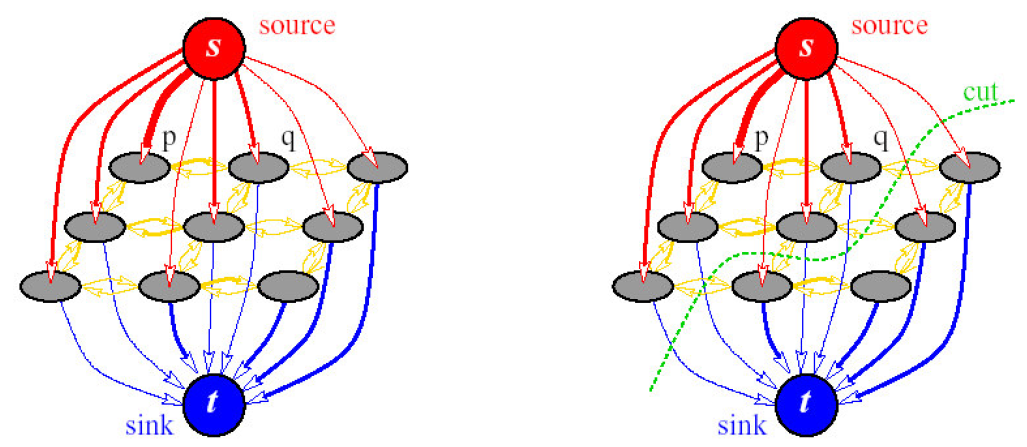
\includegraphics[width=0.8\textwidth]{Images/GC/graphcut.png} 
	\end{center}
	\caption{Forme classique d'un graphe utilisable dans les méthodes de coupes de graphe. A gauche, le graphe avec les 2 noeuds principaux $s$ et $t$. A droite, un exemple de coupe de graphe. Les arêtes en gras relient les sommets aux labels définis par la coupe.}
	\label{fig:GC_graphe}
\end{figure}

\subsubsection{Coupes minimales}

On dit que $\mathcal{C}$ est une \textbf{coupe} du graphe $\mathcal{G}$ si elle sépare $\mathcal{G}$ en deux ensembles connexes disjoints $\mathcal{S},\mathcal{T}$ tels que  
$s \in \mathcal{S}$ et $t \in \mathcal{T}$.\\
On peut alors définir la \textbf{capacité} de la coupe $\mathcal{C}$ par :
\[
	c(\mathcal{C}) = \sum_{(u,v) \in \mathcal{S} \times \mathcal{T}} c_{uv}
\]
où $c_{uv}$ est le poids assigné à l'arête $[u,v]$.\\
Une coupe de $\mathcal{G}$ est alors minimale lorsqu'il n'existe pas d'autres coupes dont la capacité est inférieure strictement. Cependant, il n'y a en général pas unicité de la coupe minimale. De nombreux algorithme permettent de calculer la coupe minimale d'un graphe via le calcul de son équivalent, le \textbf{flot maximum}. En effet, le flot maximum est facilement calculable avec des algorithmes gloutons par exemple. \\
On cherche donc à se ramener au problème de calcul de coupe minimale en affectant aux arêtes les poids suivants:
\begin{itemize}
	\item[$\bullet$] Un terme d'attache aux données, lorsque l'arête relie un sommet quelconque à $t$ ou $s$: $E_{DATA}(\lab, p)$
	\item[$\bullet$] Un terme de régularité, lorsque l'arête relie deux sommets voisins $p$ et $q$: $E_{SMOOTH}(p,q)$
\end{itemize}
On rend alors équivalents la minimisation de l'énergie $E_{TOTAL}$ et la recherche de la coupe minimale de $\mathcal{G}$.\\
Le calcul de la coupe minimale du graphe $\mathcal{G}$ ainsi construit permet de minimiser l'énergie et donc de résoudre le problème de classification.

\subsection{Application dans le cadre de la détection des nodules}

Pour appliquer des méthodes de coupes de graph au sujet qui nous intéresse, il s'agit alors de définir les fonctions d'attaches aux données et de régularisation d'une part et de construire un graphe $\mathcal{G}$ représentatif du problème d'autre part.

\subsubsection{Construction du graphe}

A chaque voxel de l'image on associe un sommet $p$ du graphe. On ajoute également $s_{IN}$ pour le label \textit{interieur} et $s_{OUT}$ pour le label \textit{exterieur}. Les sommets étant définis, il s'agit alors de les relier entre eux avec des arêtes correspondants à la réalité du problème.\\
On relie donc chaque sommets $p$ à $s_{IN}$ et $s_{OUT}$. En remarquant par ailleurs que la complexité de la minimalisation de la coupe dépend du nombre d'arêtes dans le graphe, on se contente d'appliquer un modèle de 6-connexité pour les arêtes reliant 2 sommets $p$ voisins. C'est à dire que l'affectation chaque voxel ne dépend que de l'affectation de ses 6 voisins les plus proches (2 selon chacun des 3 axes).

\subsubsection{Energies}

L'énergie d'attache aux données se calcule à partir des probabilités définies dans les parties précédentes. Celles-ci permettent d'avoir une information grossière sur la forme de l'objet à détecter. On suppose que cette probabilité est relativement proche de la réalité et on définit ainsi l'énergie d'attache aux données par :
\begin{center}
\begin{itemize}
	\item[$\bullet$] $E_{DATA}(s_{IN}, p) = f(\mathbb{P}(p \in s_{IN}))$
	\item[$\bullet$] $E_{DATA}(s_{OUT}, p) =f( \mathbb{P}(p \in s_{OUT}))$
\end{itemize}
\end{center}
$f$ peut être la fonction \textit{valeur absolue} ou \textit{carrée} par exemple.
\\
\\
L'énergie de régularisation est nulle lorsque les labels des 2 voxels voisins sont les mêmes. Dans le cas contraire, elle dépend de deux paramètres:
\begin{itemize}
	\item[$\bullet$] la différence d'intensité entre les 2 voxels doit être suffisament importante. En effet, 2 voxels voisins d'intensité similaire appartiennent certainement au même objet. La réciproque n'est par contre pas vérifiée.
	\item[$\bullet$] la localisation de leur barycentre. En effet, celui-ci est sensé appartenir à la frontière séparant les 2 objets.
\end{itemize}
En suivant les conseils de \cite{bib:seg}, nous avons utilisé les énergies suivantes:
\begin{itemize}
	\item[$\bullet$] pour la différence d'intensité: $E_{SMOOTH 1} \varpropto e^{-\frac{\Delta I^2}{2\sigma^2}}$ où $\Delta I$ est l'écart d'intensité et $\sigma$ est le paramètre de pénalisation.
	\item[$\bullet$] pour la localisation du barycentre: $E_{SMOOTH 2} \varpropto  \frac{d^2}{\sigma^2}$ où $d$ est la distance du barycentre à la frontière.
\end{itemize}
Les fonctions utilisées peuvent être quelconques à partir du moment où elles vérifient la condition de \textbf{régularité}:
\begin{equation*}
\forall i, j \{VOXEL\}, \ \ \forall l_1, l_2 \in \{LABEL\}\ \  E(i\rightarrow l_1, j\rightarrow l_1) + E(i\rightarrow l_2, j\rightarrow l_2) \leq E(i\rightarrow l_1, j\rightarrow l_2) + E(i\rightarrow l_2, j\rightarrow l_1)
\end{equation*}
Cette condition est évidemment vérifiée dans le cas précédent puisque l'égalité des labels entraine la nullité du terme de régularité et que les autres termes sont positifs ou nuls.\\
On obtient finalement une énergie de la forme:
\[
	E_{TOTAL} = \sum_{p \in \mathcal{G}} (1-\lambda)\mathbb{P}(p \in \lab(p))^2 + \lambda \sum _{p,q \in \mathcal{G} \text{ voisins}} \delta_{\lab(p) = \lab(q)} \left[ \lambda \frac{d\left(\frac{p+q}{2}, \epsilon \right)}{\sigma_d}^2 + (1-\lambda) e^{-\frac{\Delta I^2}{2\sigma_c^2}} \right]
\]
où $\delta$ est le symbole de Kronecker, $d\left(\frac{p+q}{2}, \epsilon \right)$ est la distance du barycentre de $p$ et $q$ à la frontière de l'ellipsoide $\epsilon$ et $\Delta I$ est la différence d'intensité entre $p$ et $q$. Les valeurs de $\sigma_d$ et $\sigma_c$ ont été fixées à 5 pixels et 3 d'intensité. Elles sont cependant changeables et une étude plus approfondies, réalisée à l'aide de données sur les variations d'intensité des images médicales et la taille moyenne des nodules permettrait de leur affecter une valeur plus raisonnable.

\section{Tests de segmentation}

\subsection{Test sur la détermination de l'ellipsoïde}


La méthode est robuste au bruit diffus, on a pu la tester sur des images d'ellipsoïdes bruités générés par la fonction \texttt{generate\_ellipsoïd}. Même avec un bruit important on obtient de bons résultats pour le centre et les directions des axes. Cependant, les rayons sont assez sensibles au bruit puisque ils dépendent directement du nombre de "faux positifs". Il serait intéressant de chercher une  manière de diminuer l'influence de ces "faux positifs" sur le calcul des rayons.\\\\ 
Par contre, s'il reste une zone continue de membrane non filtrée, l'ACP donne des résultat très médiocres pour les 12 paramètres.

Tant que le bruit reste diffus, l'appliction de la transformée de Hough est suffisante pour corriger l'erreur de cette étape.

\subsection{Test sur la coupe de graphe}
Pour vérifier l'efficacité de la partie segmentation, nous avons utilisé des données théoriques:
\begin{itemize}
	\item[$\bullet$] un ellipsoïde défini par avance par son centre, ses axes et ses rayons
	\item[$\bullet$] une image représentant un ellipsoide d'une certaine couleur sur un fond d'une autre couleur
	\item[$\bullet$] la loi de probabilité correspondant à la segmentation effectuée dans la première partie
\end{itemize} 
L'image et la loi de répartition ont été bruitées plus ou moins fortement pour tester la robustesse de la segmentation face à des données pas totalement fiables.\\
Les résultats suivants sont présentés sous forme de tableaux et indiquent le pourcentage de voxels mal segmentés en fonction du paramètre de régularité $\lambda$ choisi.

\begin{table}[h!]
\begin{center}
  \begin{tabular}{|c|c|c|c|c|c|c|c|c|c|c|c|}
		\hline
		$\lambda$ & 0 & 0.1& 0.2 & 0.3 & 0.4 & 0.5 & 0.6 & 0.7 & 0.8 & 0.9 & 1\\
		\hline
		$\epsilon$ (\%) & 0 & 0 & 0 & 0 & 0 & 0 & 0 & 0 & 0 & 0.7 & $\infty$\\
		\hline
\end{tabular}
\end{center}
\caption{Résultats en l'absence de bruit.}
\end{table}

\begin{table}[h!]
\begin{center}
  \begin{tabular}{|c|c|c|c|c|c|c|c|c|c|c|c|}
		\hline
		$\lambda$ & 0 & 0.1& 0.2 & 0.3 & 0.4 & 0.5 & 0.6 & 0.7 & 0.8 & 0.9 & 1\\
		\hline
		$\epsilon$ (\%) & 0 & 0 & 0 & 0 & 0 & 0 & 0 & 0 & 0 & 0.7 & $\infty$\\
		\hline
\end{tabular}
\end{center}
\caption{Résultats en bruitant la loi de répartition uniquement.}
\end{table}

\begin{table}[h!]
\begin{center}
  \begin{tabular}{|c|c|c|c|c|c|c|c|c|c|c|c|}
		\hline
		$\lambda$ & 0 & 0.1& 0.2 & 0.3 & 0.4 & 0.5 & 0.6 & 0.7 & 0.8 & 0.9 & 1\\
		\hline
        $\epsilon$ (\%) & 0.8 & 0.8 & 0.8 & 0.8 & 0.8 & 0.7 & 1.1 & 2.7 & 10.3 & 18.5 & $\infty$\\
		\hline
\end{tabular}
\end{center}
\caption{Résultats en bruitant l'image à segmenter uniquement.}
\end{table}

\begin{table}[h!]
\begin{center}
  \begin{tabular}{|c|c|c|c|c|c|c|c|c|c|c|c|}
		\hline
		$\lambda$ & 0 & 0.1& 0.2 & 0.3 & 0.4 & 0.5 & 0.6 & 0.7 & 0.8 & 0.9 & 1\\
		\hline
		$\epsilon$ (\%) & $\infty$ & 13.6 & 9.6 & 8 & 7.1 & 6.5 & 6.6 & 7.5 & 12.8 & 19.6 & $\infty$\\
		\hline
\end{tabular}
\end{center}
\caption{Résultats en bruitant l'image à segmenter et la loi de répartition.}
\end{table}

Les résultats montrent ainsi une tendance à choisir un coefficient de régularité proche de 0.5 évitant ainsi les cas extrêmes ou aucune régularité/trop de régularité sont appliquées.

\subsection{Tests pratiques}

\bibliographystyle{plain} %Style of Bibliography: plain / apalike / amsalpha / ...
\bibliography{literature} %You need a file 'literature.bib' for this.

\end{document}
